\section{Verifier-Constrained Code Generation}
\label{sec:codegen}

This section describes how \kunai lowers a filter expression into the
packet accesses, loops, and bounds checks that the Linux eBPF verifier
accepts. When nested encapsulation or a variable-length structure makes a
subsequent header's start offset vary per packet, reading a field at
that run-time offset leaves its range unprovable to the verifier. As a
result, the bytecode is rejected. The code generation below avoids it.

The difficulty is not detecting that an offset is dynamic but
lowering the read, the same way for every layer past a variable-length
one and for every protocol in the P4 subset, into a form the verifier
accepts. \kunai's code generation does this by recording each changing
header's start offset at run time (\S\ref{sec:offset}) and walking
variable-length structures such as SRv6 segments and TCP options under a
compile-time bound (\S\ref{sec:bounded}), with a verifier-compliant
bounds check before every packet read.

\subsection{Recording Header Start Offsets Explicitly}
\label{sec:offset}

\kunai records each header's start offset at run time and reads a
field as a relative offset from that start. Consider again the GTP-U
inner-IPv4 filter of \S\ref{sec:dsl}: \texttt{inner.dst} is not at a
fixed offset, since the start of the inner IPv4 changes with the outer
IPv4 length, the GTP optional fields, and the structure of the
encapsulation.

A fixed compile-time offset does not suffice: if the variable-length parts
before the field (GTP optional fields or IPv4 options) are non-empty,
it reads the wrong bytes. The offset must be computed at run time. But a
run-time offset against the native-XDP packet pointer
(\texttt{PTR\_TO\_PACKET}) is one the verifier cannot bound. The
verifier therefore cannot prove the read stays within \texttt{data\_end}
and rejects the bytecode.

\kunai detects this boundary at the resolve stage and marks every
layer after one with a variable-length layout as a run-time offset.
The generated eBPF bytecode then records each header's start offset
into a stack slot as it traverses the header at run time.
\figref{fig:layerstart} illustrates this offset recording and a
bounds-checked load that uses the recorded offset.

\begin{figure}[htbp]
  \centering
  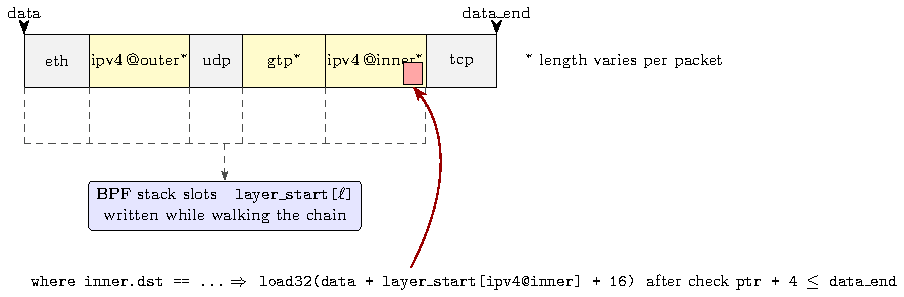
\includegraphics[width=\columnwidth]{figures/fig_layerstart.pdf}
  \caption{Recording each header's start offset into a stack slot, and
  reading \texttt{inner.dst} as a bounds-checked load at layer-start
  $+$ field offset.}
  \label{fig:layerstart}
\end{figure}

Every field access takes the same form: \kunai loads the layer's start
offset, adds the field offset and width, checks the access against
\texttt{data\_end}, loads, and compares. Because type-mismatched
comparisons and a \texttt{proto.field} reference under a repeated
protocol are already rejected at the analysis stage of
\S\ref{sec:overview}, code generation need only emit this bounds-checked
load, even for a chain whose subsequent-header start changes at run time.

\subsection{Lowering Variable-Length Structures to Bounded Bytecode}
\label{sec:bounded}

Because the element count or the length of each element changes per
packet, variable-length structures such as SRv6 segments and TCP
options cannot be walked at a fixed offset. \kunai puts the walk into a
verifier-accepted form by translating it into bytecode with a
compile-time constant bound.

\kunai generates the walk as one of two kinds of bytecode, chosen by
the bound and applied uniformly to chain quantifiers and
\texttt{any()}/\texttt{all()} aux-list walks. A small compile-time bound
within a fixed threshold is unrolled in place. A larger or unbounded one
is lowered to a
\texttt{bpf\_loop} callback with a constant
bound~\cite{bpf_loop_helper}, whose size no longer grows with the
bound; this case covers a parser-machine self-loop, an unbounded chain
quantifier, and a chain or aux-list walk past the threshold.
An SRv6 segment walk and a large MPLS stack take the same lowering.

Algorithm~\ref{alg:walk} gives the shared skeleton; the two lowerings
below instantiate its \textsc{stop}, \textsc{stride}, and \textsc{step}
steps, each emitted by its own generator.

\begin{algorithm}[htbp]
  \caption{Bounded walk skeleton; \textsc{stop}, \textsc{stride}, and
  \textsc{step} are instantiated per structure.}
  \label{alg:walk}
  \begin{algorithmic}[1]
    \Require $data,\ data\_end,\ base,\ cap$; \textsc{stop}, \textsc{stride}, \textsc{step} per structure
    \State $r \gets \bot$;\ $off \gets base$
    \For{$i \gets 0$ \textbf{to} $cap-1$} \Comment{$cap$: compile-time bound}
      \State \textbf{if} $\textsc{stop}(i, off)$ \textbf{then break} \Comment{count reached, or end/END/malformed}
      \State $ptr \gets data + off$
      \State \textbf{if} $ptr + w > data\_end$ \textbf{then break} \Comment{$w$: bytes read; bounds check}
      \State $r \gets \textsc{step}(ptr)$; \textbf{break if} $r$ decides \Comment{compare, or record option}
      \State $off \gets off + \textsc{stride}(ptr)$ \Comment{constant, or this option's length}
    \EndFor
    \State \Return $r$
  \end{algorithmic}
\end{algorithm}

\kunai instantiates this skeleton in two ways, chosen by the structure
rather than the protocol. A \emph{counted aux-list walk} handles a list
of fixed-size elements with a run-time count, such as the SRv6 segment
list: \textsc{stop} is $i \geq count$, \textsc{stride} is the constant
element width, and \textsc{step} compares the element field to the
target and decides the walk on a match. For the SRv6 segment filter of
\S\ref{sec:dsl}, \texttt{base = srh\_start + SRH\_FIXED\_SIZE},
\texttt{stride = width = 16}, \texttt{count = last\_entry + 1} (the SRv6
parser's segment-walk seed in \S\ref{sec:p4subset}), and
\texttt{target = fc00::1}.

A \emph{TLV self-loop} handles options that differ in kind and length,
such as TCP options, where a reference like
\texttt{tcp.\allowbreak options.\allowbreak MSS.\allowbreak value} sits
at no fixed offset. Here \textsc{stride} is each option's length,
read at the cursor; \textsc{stop} fires when the cursor reaches the end
of the options, on an END option, on a malformed option (\texttt{len < 2}
or \texttt{cursor + len > options\_end}), or at the iteration bound; and
\textsc{step} dispatches on the option kind and records the position of
the referenced option, which the \texttt{where} clause then reads after
the walk. An option field is loaded only after checking that its option
header stays within the packet window.

In either instantiation, and in either the fixed-unrolling or the
\texttt{bpf\_loop} form, the bound is a compile-time constant and a
bounds check precedes every packet load. The verifier can therefore
confirm both the loop bound and the range of every packet access.

So that the generated bytecode is accepted across kernel versions,
\kunai avoids instructions available only on newer versions. For
byte-order conversion, for example, it uses the \texttt{BPF\_END}
instruction, available on older versions, rather than the
\texttt{BSWAP} instruction introduced in 6.6~\cite{bpf_isa}.

These two patterns are not specific to \kunai but are what a
verifier-safe lowering of nested, variable-length filters requires.
\emph{Recorded-base addressing} reads each field as a recorded
layer-start base plus a static offset, spilling the base to a stack slot
during traversal, which makes an otherwise unprovable run-time read
provable. \emph{Constant-bounded scanning} bounds every variable-length
walk by a compile-time cap, unrolled when small and lowered to a
\texttt{bpf\_loop} callback when large; both the trip count and each
read are therefore provable. Only the base, run-time or compile-time constant,
varies between reads; the read shape is uniform, and \kunai selects the
lowering from the structure's shape, not its protocol name. GTP-U,
SRv6, Geneve, and TCP options therefore need no per-protocol code in
the generator.
